% !TeX TS-program = xelatex

%\documentclass{beamer}
\documentclass[xcolor=dvipsnames, professionalfonts, aspectratio=169, 11pt]{beamer}

\usepackage{multicol}
\usepackage{tikz}
\usetikzlibrary{automata, positioning, arrows}
\usepackage{dblfnote}
\usepackage{float}
\usepackage{setspace}
\usepackage{xecolor}
\usepackage{amsmath}
\usepackage{caption}
\usepackage{subcaption}



\usepackage{wrapfig}
%---------------------------------------------------------------%
\usepackage{lipsum}


%Set the slide theme
%Change to meet your taste
% Madrid, Copenhagen, Berlin, ... works

\usetheme[compress]{Ilmenau}
%\usetheme{AnnArbor}
%\usetheme{Frankfurt}
%\usetheme{CambridgeUs}
%\usetheme{metropolis}
\makeatletter
\beamer@theme@subsectionfalse
\makeatother


%\usefonttheme[onlymath]{serif} %Change the math font

\usepackage[
extrafootnotefeatures,
localise=on,
mathdigits=default,
inlinemathdigits=default,
displaymathdigits=default % persian
]{xepersian}
\settextfont{XB Niloofar}
\setlatintextfont{Junicode}
% \settextfont{XB Roya}


\usecolortheme{beaver}
\setbeamercolor{section number projected}{bg=red,fg=white}
\setbeamercolor*{item}{fg=red}

%% green theme
%\usecolortheme{spruce}
%\setbeamercolor{section number projected}{bg=OliveGreen,fg=white}
%\setbeamercolor*{item}{fg=OliveGreen}

%\usecolortheme[named=green]{structure}
%\setbeamercolor{normal text}{fg=blue}\usebeamercolor*{normal text}

% ---------------------------------------
% font
% ---------------------------------------

\newfontfamily\TitrFont[Path={/home/reza/.fonts/}, Scale=1]{IRTitr.ttf}
\newfontfamily\NormalFont[Path={/home/reza/.fonts/}, BoldFont={IRLotusICEE_Bold.ttf}, BoldItalicFont={IRLotusICEE_BoldIranic.ttf}, ItalicFont={IRLotusICEE_Iranic.ttf},Scale=1.2]{IRLotusICEE.ttf}

\newif\ifirfonts

\makeatletter
% تعریف قلم فارسی و انگلیسی و مکان قلم‌ها
\ifirfonts
\settextfont[Path={/home/reza/.fonts/}, BoldFont={IRLotusICEE_Bold.ttf}, BoldItalicFont={IRLotusICEE_BoldIranic.ttf}, ItalicFont={IRLotusICEE_Iranic.ttf},Scale=1.2]{IRLotusICEE.ttf}
% LiberationSerif or FreeSerif as free equivalents of Times New Roman
\setlatintextfont[Path={/home/reza/.fonts/}, BoldFont={LiberationSerif-Bold.ttf}, BoldItalicFont={LiberationSerif-BoldItalic.ttf}, ItalicFont={LiberationSerif-Italic.ttf},Scale=1]{LiberationSerif-Regular.ttf}
% چنانچه می‌خواهید اعداد در فرمول‌ها، انگلیسی باشد، خط زیر را غیرفعال کنید
% و گزینهٔ displaymathdigits=persian را از خط ۱۰۹ حذف کنید.
%\setdigitfont[Path={/home/reza/.fonts/}, Scale=1.2]{IRLotusICEE.ttf}
% تعریف قلم‌های فارسی و انگلیسی اضافی برای استفاده در بعضی از قسمت‌های متن
\setiranicfont[Path={/home/reza/.fonts/}, Scale=1.3]{IRLotusICEE_Iranic.ttf}				% ایرانیک، خوابیده به چپ
\setmathsfdigitfont[Path={/home/reza/.fonts/}]{IRTitr.ttf}
\defpersianfont\titlefont[Path={/home/reza/.fonts/}, Scale=1]{IRTitr.ttf}
% برای تعریف یک قلم خاص عنوان لاتین، خط بعد را فعال و ویرایش کنید و خط بعد از آن را غیرفعال کنید.
% \deflatinfont\latintitlefont[Scale=1]{LiberationSerif}
\font\latintitlefont=cmssbx10 scaled 2300 %cmssbx10 scaled 2300

\else
\settextfont{XB Niloofar}
\setlatintextfont{Junicode}
% چنانچه می‌خواهید اعداد در فرمول‌ها، انگلیسی باشد، خط زیر را غیرفعال کنید
% و گزینهٔ displaymathdigits=persian را از خط ۱۰۹ حذف کنید.
%\setdigitfont{XB Niloofar}
% \setdigitfont{Junicode}
% تعریف قلم‌های فارسی و انگلیسی اضافی برای استفاده در بعضی از قسمت‌های متن
% \setmathsfdigitfont{XB Titre}
\defpersianfont\titlefont{XB Titre}
\deflatinfont\latintitlefont[Scale=1.1]{Junicode}
\fi
\makeatother

% برای استفاده از قلم نستعلیق خط بعد را فعال کنید.
% \defpersianfont\nastaliq[Scale=1.2]{IranNastaliq}



% ---------------------------------------
% frame options
% ---------------------------------------

% \setbeamerfont{section name}{family=\TitrFont}
\setbeamerfont{section title}{family=\TitrFont,size=\huge}
\setbeamerfont{subsection title}{size=\Large}
% \setbeamerfont{frametitle}{family=\TitrFont}
\setbeamerfont{title}{family=\TitrFont}
\setbeamerfont{subtitle}{family=\NormalFont}

% \setbeamertemplate{section in toc}[circle]
% \setbeamertemplate{frametitle continuation}{\gdef\beamer@frametitle{}} % framebreaks without numbering
\setbeamertemplate{frametitle}[default][center]% align the frametitle to the center
\setbeamertemplate{caption}[numbered]{}% Number float-like environments
\setbeamertemplate{itemize item}{\scriptsize\raise1.25pt \hbox{\donotcoloroutermaths$\blacktriangleleft$}} % Correct the bullet for RTL texts
\setbeamertemplate{enumerate item}[circle] % ball or circle

%\setbeamersize{text margin left=5mm,text margin right=10mm}




% ---------------------------------------
% frame options
% ---------------------------------------

% \setbeamerfont{section name}{family=\TitrFont}
\setbeamerfont{section title}{family=\TitrFont,size=\huge}
\setbeamerfont{subsection title}{size=\Large}
% \setbeamerfont{frametitle}{family=\TitrFont}
\setbeamerfont{title}{family=\TitrFont}
\setbeamerfont{subtitle}{family=\NormalFont}

% \setbeamertemplate{section in toc}[circle]
% \setbeamertemplate{frametitle continuation}{\gdef\beamer@frametitle{}} % framebreaks without numbering
\setbeamertemplate{frametitle}[default][center]% align the frametitle to the center
\setbeamertemplate{caption}[numbered]{}% Number float-like environments
\setbeamertemplate{itemize item}{\scriptsize\raise1.25pt \hbox{\donotcoloroutermaths$\blacktriangleleft$}} % Correct the bullet for RTL texts
\setbeamertemplate{enumerate item}[circle] % ball or circle

%\setbeamersize{text margin left=5mm,text margin right=10mm}


%%% تصحیح  \subsection و \subsubsection در فهرست مطالب
\makeatletter
\expandafter\let\csname beamer@@tmpop@subsection in toc@default\endcsname\relax
\expandafter\let\csname beamer@@tmpop@subsubsection in toc@default\endcsname\relax
\defbeamertemplate*{subsection in toc}{default}
{\leavevmode\rightskip=1.5em\inserttocsubsection\par}

\defbeamertemplate*{subsubsection in toc}{default}
{\leavevmode\normalsize\usebeamerfont{subsection in toc}\rightskip=3em%
	\usebeamerfont{subsubsection in toc}\inserttocsubsubsection\par}
\makeatother
%%%%%%%%%%%%%%%%%%%%%%%%%%%%%%%

\makeatletter
\defbeamertemplate{section in toc}{RtlTocBall}{
	\leavevmode\leftskip=2.75ex
	\llap{
		\normalsize
		\begin{pgfpicture}{-1ex}{-0.7ex}{1ex}{1ex}
			\pgftext{\beamer@usesphere{section number projected}{tocsphere}}
			\pgftext{
				\usebeamerfont*{section number projected}
				\usebeamercolor{section number projected}
				\color{fg!90!bg}
				\hspace{-0.8em}
				\inserttocsectionnumber}
		\end{pgfpicture}
		\kern1.25ex}
	\raggedleft \inserttocsection\par
}
[action]
{\setbeamerfont{section number projected}{size=\scriptsize}}

\defbeamertemplate{subsection in toc}{RtlTocBall}
{\leavevmode\leftskip=5ex
	\hspace{1.5em}\llap{\raise0.1ex\beamer@usesphere{subsection number projected}{bigsphere}\kern1ex}
	\raggedleft \inserttocsubsection\par
}

\setbeamertemplate{subsubsection in toc}{
	\setRTL \rightskip=3ex\myitem
	\inserttocsubsection\par
}

\setbeamertemplate{sections/subsections in toc}[RtlTocBall]
\makeatother

\makeatletter
\newcommand{\RTList}{\raggedleft\rightskip\@totalleftmargin}
\newenvironment{shomarei}[1][]{\begin{enumerate}[#1]\RTList}{\end{enumerate}}
\newenvironment{moredi}[1][]{\begin{itemize}[#1]\RTList}{\end{itemize}}
\makeatother


%%% تصحیح دستورات \frametitle و \framesubtitle برای قرار دادن عنوان و زیرعنوان یک frame استفاده کنیم:
\makeatletter
\define@key{beamercolbox}{left}[0pt]{\def\beamer@colbox@rs{0pt}\def\beamer@colbox@ls{#1 plus1fill}}
\makeatother


\makeatother

% hide navigation bar
\beamertemplatenavigationsymbolsempty

% fix allowframebreaks numbering
\setbeamertemplate{frametitle continuation}{ - \insertcontinuationcount}

\makeatletter
% reset footnot counter per new page
% \@newctr{footnote}[page]
\makeatother


\makeatother

% hide navigation bar
\beamertemplatenavigationsymbolsempty

% fix allowframebreaks numbering
\setbeamertemplate{frametitle continuation}{ - \insertcontinuationcount}

\makeatletter
% reset footnot counter per new page
% \@newctr{footnote}[page]
\makeatother


% دستور های لازم برای تعریف ترجمهٔ دستورات الگوریتم
\makeatletter
% تعریف محیط بدون headline
\newenvironment{withoutheadline}{
	\setbeamertemplate{headline}[default]
	\def\beamer@entrycode{\vspace*{-\headheight}}
}{}
\makeatother

% برای درج عدد به جای شکل در beamer
\setbeamertemplate{bibliography item}{\insertbiblabel}

\renewcommand{\sectionname}{قسمت}
\renewcommand{\subsectionname}{زیرقسمت}
\def\subsubsectionname{\translate{Subsubsection}}
\def\insertsubsubsectionnumber{\arabic{subsubsection}}
%\def\subsubsectionpage{\usebeamertemplate*{subsubsection page}}
\AtBeginSection{\frame{\sectionpage}}
%\AtBeginSubsection{\frame{\subsectionpage}}
%\AtBeginSubsubsection{\frame{\subsubsectionpage}}


\def\Put(#1,#2)#3{\leavevmode\makebox(0,0){\put(#1,#2){#3}}}
















%%%%%%%%%%%%%%%%%%%%%%%%%%%%%%%%%%%%%%

%%% تصحیح مشکل پانویس footnote

\makeatletter
\bidi@undef\beamer@@tmpop@footnote@default



% برای شفاف کردن مواردی که در
%\setbeamercovered{transparent}

\setbeamertemplate{frametitle}
{
	\nointerlineskip
	\begin{beamercolorbox}[sep=0.0cm,ht=1.6em,wd=\paperwidth]{frametitle}
		\vbox{}\vskip-1ex%
		\centering
		%	\raisebox{-1em}{
\includegraphics[height=1.6em]{./img/eng-logo.png}} \hfill
		{  \strut\insertframetitle\strut}
		%		\hfill		
\includegraphics[height=1.6em]{./img/logo.png}
		\vskip+0.2ex %		\vskip-0.8ex%
	\end{beamercolorbox}
}


\makeatletter
\setbeamertemplate{footline}
{
	\leavevmode%
	\hbox{\tiny%\fontsize{7}{8}\selectfont%
		\begin{beamercolorbox}[wd=.3\paperwidth,ht=2.25ex,dp=1ex,center]{author in head/foot}
			\hspace*{1ex}\usebeamerfont{author in head/foot}\insertshortauthor~~\beamer@ifempty{\insertshortinstitute}{}{(\insertshortinstitute)}\hspace*{1ex}
		\end{beamercolorbox}%
		\begin{beamercolorbox}[wd=.5\paperwidth,ht=2.25ex,dp=1ex,center]{title in head/foot}
			\usebeamerfont{title in head/foot}\insertshorttitle
		\end{beamercolorbox}%
		\begin{beamercolorbox}[wd=.2\paperwidth,ht=2.25ex,dp=1ex,right]{date in head/foot}
			\hfill
			\usebeamerfont{date in head/foot}\insertshortdate{}
			\hfill % \hspace*{4ex}% original: 2ex
			\inserttotalframenumber / \insertframenumber{} \hspace*{1ex}% original: 2ex
	\end{beamercolorbox}}%
	\vskip0pt%
}
\makeatother
\makeatletter
\setbeamerfont{frametitle}{size=\small}
\makeatother
%% simple headline for one row sectino name and one row subsection name
%\setbeamertemplate{headline}{
	%	\begin{beamercolorbox}[wd=\paperwidth,ht=2.5ex,dp=1.125ex]{section in head/foot}%
		%		\hspace{3ex}{\insertsectionhead}
		%	\end{beamercolorbox}
	%	\begin{beamercolorbox}[ht=2.5ex,dp=1.125ex,leftskip=.3cm,rightskip=.3cm plus1fil]{subsection in head/foot}
		%		\usebeamerfont{subsection in head/foot}\insertsubsectionhead
		%\end{beamercolorbox}}
		
		%% add section navigation above frame title (miniframe style)
		\setbeamertemplate{headline}{%
			\begin{beamercolorbox}{section in head/foot}
				\vskip0pt\insertnavigation{\paperwidth}\vskip2pt
			\end{beamercolorbox}%
		}
		% add section navigation above frame title
		%\setbeamertemplate{headline}
		%{
			%	\begin{beamercolorbox}{section in head/foot}
				%		\vskip2pt\insertsectionnavigationhorizontal{\textwidth}{}{}\vskip2pt
				%	\end{beamercolorbox}
			%}
		\setbeamertemplate{section in head/foot}{\color{fg}\insertsectionhead}
		\setbeamertemplate{section in head/foot shaded}{\color{fg!50!bg}\insertsectionhead}
		\setbeamercolor{section in head/foot}{fg=white}
		
		%%% can add logo to section frame
		%% \newcommand{\secimage}{example-image-a}
		%%% can change in document with
		%% \renewcommand{\secimage}{example-image-b}
		%\AtBeginSection[]{
			%	\begin{frame}
				%		\vfill
				%		\centering
				%%       \includegraphics[width=4cm]{\secimage}
				%		\begin{beamercolorbox}[sep=8pt,center,shadow=true,rounded=true]{title}
					%			\usebeamerfont{title}\insertsectionhead\par%
					%		\end{beamercolorbox}
				%		\vfill
				%	\end{frame}
			%}
		
		
		\title
[پیش‌بینی RUL دستگاه‌های دوار با استفاده از شبکه عصبی ترنسفرمر بر بستر FPGA]
{شتاب‌دهی سخت‌افزاری پیش‌بینی عمر باقی‌مانده مفید دستگاه‌های دوار با استفاده از شبکه عصبی ترنسفرمر بر بستر FPGA}
		
		\author[رضا آدینه پور]{رضا آدینه پور}
		%\subtitle{ارائهٔ نمونه‌ای}
		\institute[دانشگاه صنعتی امیرکبیر]{
			استاد راهنما: جناب آقای دکتر مرتضی صاحب الزمانی\\
			دانشکدهٔ مهندسی کامپیوتر  /  دانشگاه صنعتی امیرکبیر \\
			\href{mailto:adinepour@aut.ac.ir}{\texttt{adinepour@aut.ac.ir}}
		}
		%\date{زمستان ۱۳۹۹}
		\subject{مهندسی کامپیوتر}
		
		% \AtBeginDocument{
			\makeatletter
			\hypersetup{
				pdftitle={نمونه ارائه فارسی با beamer},
				pdfauthor={رضا آدینه پور},
				pdfsubject={Thesis in {نمونه ارائه فارسی با beamer}},
				%        pdfkeywords={\@latinkeywords},
				pdfdirection={R2L}
			}
			\makeatother
			% }
		
		\titlegraphic{
			\vspace{-2cm}
			\makebox[0.9\paperwidth]{
				
\includegraphics[height=1.9cm]{./img/logo-ce.png}
				\hfill
				
\includegraphics[height=2cm]{./img/logo-aut.png}
				\vspace{5 mm}
			}
		}

%-------------------------------------------------------------------------------
% Seetings to force Beamer works with Xepersian and RTL typesetting
%-------------------------------------------------------------------------------
%\raggedleft

% For right to left lists (itemize and enumerate)
\makeatletter
%\newcommand{ \RTList}{\raggedleft\rightskip\@totalleftmargin} 
\makeatother
% Correct the bullet for RTL texts
\setbeamertemplate{itemize item}{\scriptsize\raise1.25pt%
 \hbox{\donotcoloroutermaths$\blacktriangleleft$}} 

% To force beamer use numbering in captions
\setbeamertemplate{caption}[numbered]{}% Number float-like environments



%--------------------------------------------------------------------------------


\begin{document}
	
\begin{persian}
%------------------------------------------
% Title page
%------------------------------------------
\begin{frame}
\maketitle
\end{frame}

 \begin{frame}
	\frametitle{فهرست}
	% \raggedright
	\tableofcontents
\end{frame}








\section{مقدمه}
\begin{frame}
	\frametitle{مقدمه}
	\textbf{چرا بلبرینگ؟}
	
	\setbeamercolor{alerted text}{fg=red}
	\setbeamerfont{alerted text}{series=\bfseries}
	\setbeamercovered{transparent}
		

	% \raggedleft
	\begin{enumerate}
		\item یکی از مهم‌ترین و پرکاربردترین قطعه صنعتی است و در تمام ابزار‌های صنعتی حضور گسترده دارد
		\begin{itemize}
			\item خودرو‌ها
			\item توربین‌ها
			\item ژنراتور‌ها
		\end{itemize}
		\item به دلیل بار زیاد، زودتر از قطعات دیگر تخریب می‌شوند
	\end{enumerate}
		

%	\begin{figure}
%		\vspace{0em}
%		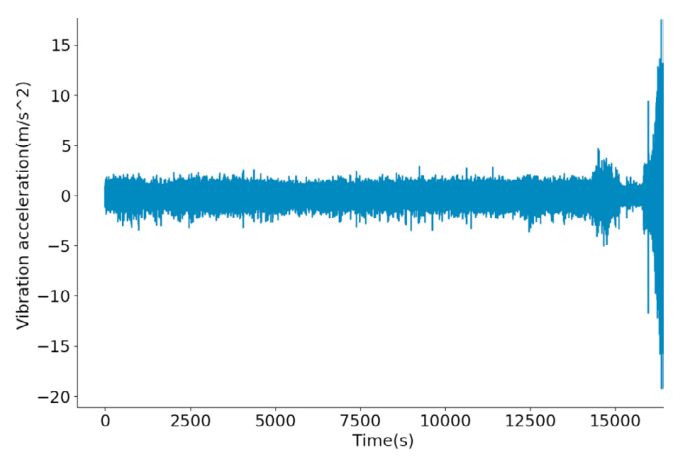
\includegraphics[height=0.4\textheight]{img/img1.png}
%		\caption{سیگنال لرزش یک بلبرینگ}
%	\end{figure}
		
	\begin{figure}
		\centering
		\begin{subfigure}[b]{0.4\textwidth}
			\centering
			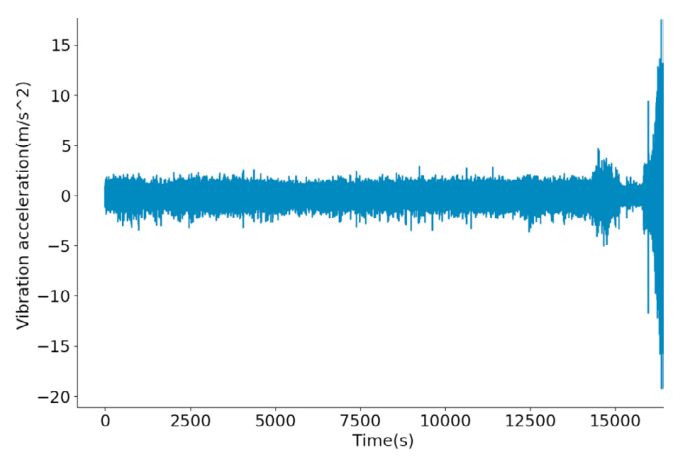
\includegraphics[width=\textwidth]{img/img1.png}
			\caption{$y=x$}
			\label{fig:y equals x}
		\end{subfigure}
		\hspace{0cm}
		\begin{subfigure}[b]{0.3\textwidth}
			\centering
			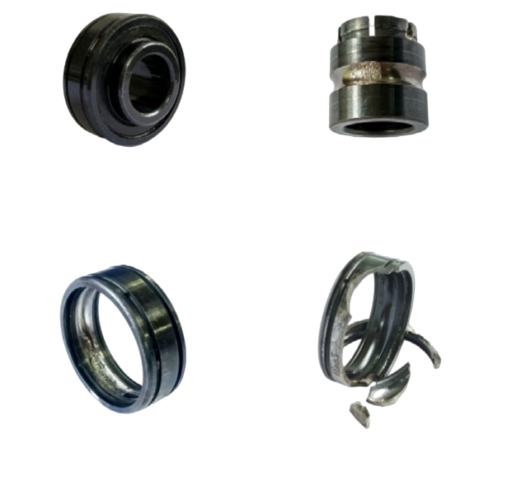
\includegraphics[width=\textwidth]{img/img2.png}
			\caption{$y=3\sin x$}
			\label{fig:three sin x}
		\end{subfigure}
		\hspace{0cm}
	\end{figure}
\end{frame}








\section{مفاهیم اولیه}

\subsection{اولین زمان پیش‌بینی (FPT) و زمان پایان عمر (EOL)}
\begin{frame}
	\frametitle{اولین زمان پیش‌بینی (FPT) و زمان پایان عمر (EOL)}
	
	
	\begin{multicols}{2}
		\begin{figure}
			\vspace{0em}
			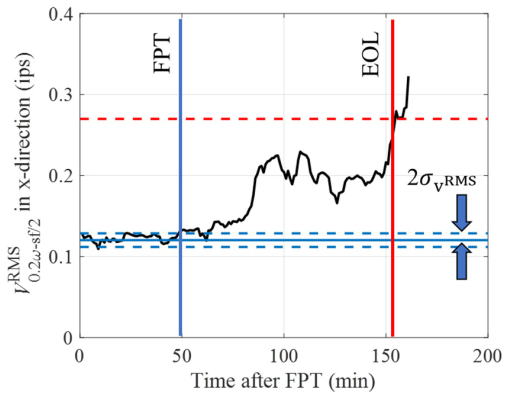
\includegraphics[height=0.6\textheight]{img/img3.png}
			\caption{بازه زمانی عمر سیستم}
		\end{figure}
		
		\begin{enumerate}
			\item :FPT اولین زمانی که علائم خرابی در سیگنال ظاهر می‌شود
			\begin{itemize}
				\item معمولا سیستم داغ می‌شود و به لرزش می‌افتد
				\item نویز سیستم زیاد می‌شود
			\end{itemize}
			\item :EOL پایان عمر سیستم
		\end{enumerate}
		
		\pause
		\begin{eqnarray}
		V_{0.2\omega-\frac{sf}{2	}}^{RMS}=\sqrt{\sum_{f=0.2\omega}^{\frac{sf}{2}}\frac{|V(f)|^2}{2}} , sf=25.6 KHz
		\end{eqnarray}
		
		\begin{eqnarray}
		RUL(t)=T_{EOF} - T_{FPT}
		\end{eqnarray}
		
%		\begin{theorem}<1->[Pythagoras]
%			$$ RUL(t)=EOL(t)-FPT(t) $$
%		\end{theorem}
		
	\end{multicols}
	
%	\begin{figure}
%		\vspace{0em}
%		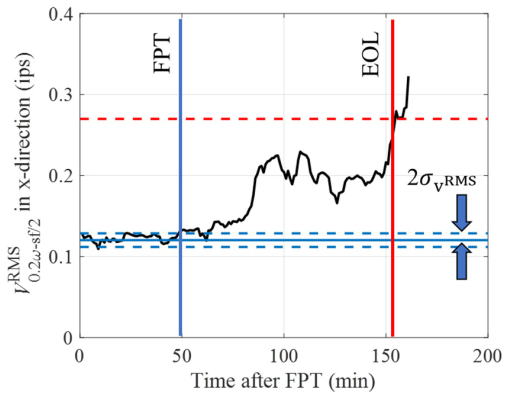
\includegraphics[height=0.6\textheight]{img/img3.png}
%		\caption{سیگنال لرزش یک بلبرینگ}
%	\end{figure}


%\begin{minipage}{0.45\textwidth}
%	\begin{enumerate}
%		\item First item \\
%		This is the second line in item and this may extend to third if long
%		\item second item\ldots
%	\end{enumerate}
%\end{minipage}%
%
%\hfill
%
%\begin{minipage}{0.45\textwidth}
%	\begin{tabular}{\textwidth}
%		
%		\begin{figure}
%			\vspace{0em}
%			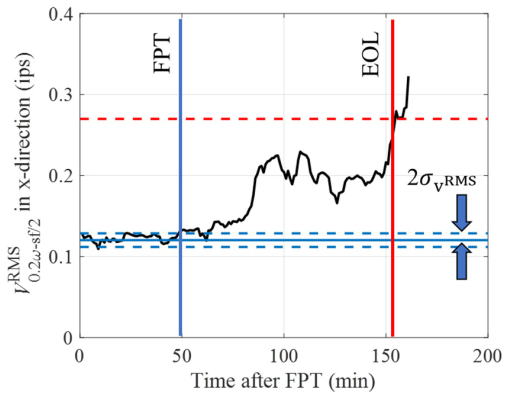
\includegraphics[height=0.6\textheight]{img/img3.png}
%			\caption{سیگنال لرزش یک بلبرینگ}
%		\end{figure}	
%	\end{tabular}
%\end{minipage}%
%	
	
	
	
%	
%	\begin{columns}[onlytextwidth]
%		\setbeamercolor{alerted text}{fg=red}
%		\setbeamerfont{alerted text}{series=\bfseries}
%		\setbeamercovered{transparent}
%		\begin{column}{.4\textwidth}
%			% \raggedleft
%			\begin{enumerate}
%				\item نمونه از یک لیست دولایه در کنار یک تصویر
%				\begin{enumerate}[<1>]
%					\item در این لیست موارد زیادی می‌تواند قرار بگیرد
%					\item مثلاً
%					\item $\cdots$
%					
%				\end{enumerate}
%			\end{enumerate}
%		\end{column}
%		
%		
%		
%		
%		\begin{column}{.6\textwidth}
%			% \raggedleft
%			\begin{enumerate}
%				\item این مورد برای یک ترکیب دولایه ای آماده شده
%				\begin{enumerate}
%					\item<1> این مورد فقط در قسمت اول دیده می‌شود
%					\item \alert<2>{این مورد تأکیدی در صفحهٔ دوم دیده می‌شود}
%					\item<1> موارد بیشتر
%					
%				\end{enumerate}
%			\end{enumerate}
%			\begin{figure}
%				% \includegraphics[width=\textwidth]{./img/social-sais.jpg}
%				\vspace{-1em}
%				
\includegraphics[height=0.35\textheight]{img/logo-ce.png}
%				\caption{اولین تصویر }
%			\end{figure}
%		\end{column}
%		% \begin{column}{.01\textwidth}\end{column}
%	\end{columns}
\end{frame}











\subsection{عمر باقی‌مانده مفید}
\begin{frame}
	\frametitle{عمر باقی‌مانده مفید}
	
	فرایند تخریب و عمر باقی مانده مفید یک سیستم $\equiv$ تابعی خطی با شیب 45-
	
	
	\begin{figure}
		\centering
		\begin{subfigure}[b]{0.45\textwidth}
			\centering
			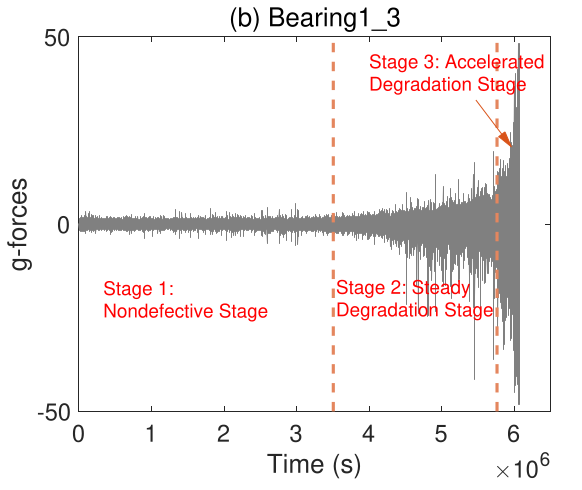
\includegraphics[width=\textwidth]{img/img4.png}
			\caption{سیگنال ارتعاشات بلبرینگ}
			\label{سیگنال ارتعاشات بلبرینگ}
		\end{subfigure}
		\hspace{0cm}
		\begin{subfigure}[b]{0.5\textwidth}
			\centering
			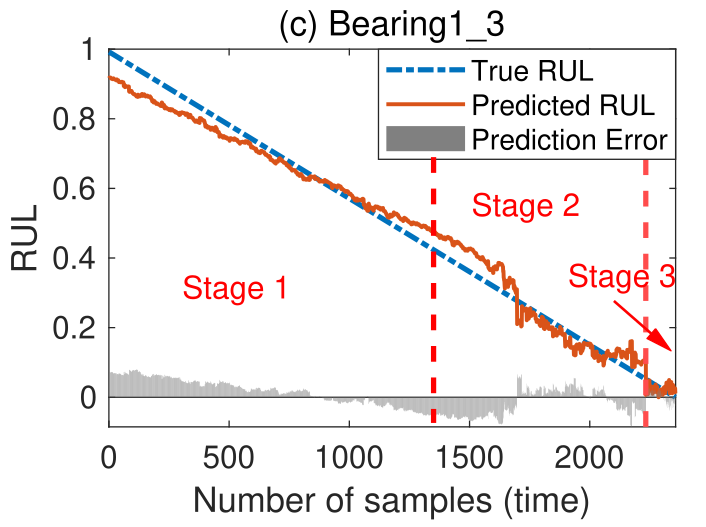
\includegraphics[width=\textwidth]{img/img5.png}
			\caption{تابع تخریب RUL}
			\label{تابع تخریب RUL}
		\end{subfigure}
		\hspace{0cm}
	\end{figure}
	
	
	
%	\begin{table}
%		\caption{حالت‌های معروف برای مدل مارکوف}
%		\vspace{0em}
%		\small
%		\begin{tabular}{|c|c|c|}
%			\hline
%			\textbf{حالت‌ها}       & \textbf{زمان پیوسته}       & \textbf{زمان گسسته}        \\
%			\hline
%			\textbf{وضعیت گسسته}  & فرایند مارکوف              & زنجیره مارکوف              \\
%			\hline
%			\textbf{وضعیت پیوسته} & فرایند مارکوف وضعیت پیوسته & زنجیره مارکوف وضعیت پیوسته \\
%			\hline
%		\end{tabular}
%	\end{table}
	
\end{frame}








\subsection{ساختار ترنسفرمر}
\begin{frame}
	\frametitle{ساختار ترنسفرمر}
	
	
	\begin{multicols}{2}
		
		\begin{figure}
			\vspace{0em}
			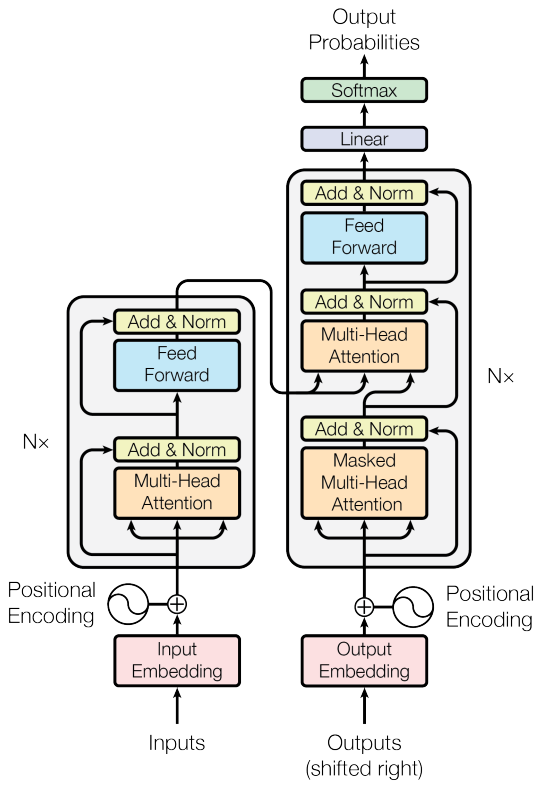
\includegraphics[height=0.8\textheight]{img/img6.png}
			%\caption{بازه زمانی عمر سیستم}
		\end{figure}
	
	\begin{enumerate}
		\begin{latin}
			\item Encoder
			\begin{itemize}
				\item Multi-Head Attention
				\item Feed Forward
			\end{itemize}
			\item Decoder
			\begin{itemize}
				\item Multi-Head Attention
				\item Feed Forward
				\item Linear
				\item Softmax
			\end{itemize}
		\end{latin}
	\end{enumerate}
	
	\end{multicols}
	
	
	
	
	
	
	
	
\end{frame}


















% To adjust the paragraphs in RTL
\everypar{\rightskip\rightmargin}
%-------------------------------------------------------------------------------
\section{مبانی}
\subsection{متن ساده}
\begin{frame}

این یک نمونه بسیار ساده از اسلاید است که با بیمر و زی‌پرشین ساخته شده‌است.

از فونت آزاد Roya XB برای این اسلاید استفاده شده‌است. این فونت در اینترنت موجود است و باید روی کامپیوتر شما نصب شده باشد یا در فولدر قابل دسترس برای زی‌لاتک باشد

تنظیمات اندکی در بخش آغازین برای اصلاح لیست‌ها و عنوان اسلایدها اضافه شده است. همچنین نحوه شماره‌گذاری تصاویر و جدول‌ها تنظیم شده‌است.

بسیاری از تم‌های استاندارد بیمر با این الگو قابل استفاده است.

استفاده از پانویس توصیه نمی شود. سفارش می‌شود که جدول فهرست مطالب به شکل دستی باشد. این اسلاید با بسیاری از تم‌های بیمر کار میکند اگرچه ممکن است اشکالاتی وجود داشته باشد.
\end{frame}

%-------------------------------------------------------------------------------
%\section{لیست‌های بدون شماره و با شماره}
%%-------------------------------------------------------------------------------
%\begin{frame}{استفاده از لیست‌های بدون شماره}
%
%استفاده از محیط لیست‌های بدون شماره در این‌جا آورده شده است. به نحوه راست چین نمودن لیست در فایل tex دقت نمایید.
%\begin{itemize}\RTList
%	\item مورد اول
%	\item مورد دوم
%	\item مورد سوم که یک متن طولانی تر است\\ ما چند خط در اینجا آورده‌ایم
%	\item مورد آخر
%\end{itemize}
%\end{frame}
%
%%-------------------------------------------------------------------------------
%\begin{frame}{استفاده از محیط شماره‌گذاری}
% استفاده از محیط لیست (itemize) و شماره‌گذاری (enumerate) بصورت ترکیبی در این‌جا آورده شده است
% \begin{enumerate}\RTList
%      \item سطح یک - مورد اول
%	      \begin{itemize}\RTList
%	      		\item  سطح دوم - مورد اول
%	     		 \item  سطح دوم - مورد دوم
%	      \end{itemize}
%      \item سطح یک - مورد دو
%      \item سطح یک - مورد سه
% \end{enumerate}
%
%این یک پاراگراف ساده پارسی بعد از محیط شماره‌گذاری است.
%\end{frame}
%
%
%%-------------------------------------------------------------------------------
%\begin{frame}{استفاده از رنگ و متن انگلیسی در اسلاید پارسی}
%در این اسلاید نحوه استفاده از رنگ از بسته xecolor و نیز محیط LTR برای نوشتن متن پارسی آمده‌است.
%\vspace{1cm}
%
%{\xecolor{green}
%	استفاده از \textbf{رنگ} و متن انگلیسی در داخل اسلاید پارسی
%}
%\vspace{1cm}
%{\xecolor{red}
%	\begin{LTR}
%		This is an English Paragraph inside a Persian slide!\\
%		Another line of latin text.
%	\end{LTR}
%}
%
%\end{frame}
%
%
%%-------------------------------------------------------------------------------
%\begin{frame}
%\frametitle{معادلات ریاضی}
%چنانکه ملاحظه می‌شود عنوان در بیمر + زی‌پرشین به درستی کار می‌کند
%\vspace{2cm}
%\begin{equation}
%\int_{a}^{b} f(x)dx = \frac{\lambda x^2 + \gamma x + \beta}{1+\sum_{n=1}^{m+2} 3 \alpha x^2 +x_n \sin(2 x_n -1)}
%\end{equation}
%
%\end{frame}
%
%%------------------------------------------
%% Tables and Pictures
%%------------------------------------------
%\section{کار با تصویر و جدول}
%
%%------------------------------------------
%\begin{frame}
%\frametitle{شکل‌ها}
%\begin{figure}
%	\centering
%	
\includegraphics[width=0.4\linewidth]{settings-blue.pdf}
%	\caption[نمونه تصویر]{چگونگی درج یک تصور در بیمر+زی‌پرشین}
%	\label{fig:pic1}
%\end{figure}
%\end{frame}
%
%
%%-------------------------------------------------------------------------------
%\begin{frame}{جداول در بیمر و زی‌پرشین}
%\begin{table}
%\caption{نمونه متن در جدول فارسی}
%\begin{tabular}{|c|c|c|c|}
%	\hline 
%خانه اول	& خانه وسط جدول &خانه سمت راست    \\ 
%	\hline 
%ردیف دوم	&  ردیف دوم خانه دوم& ردیف دوم خانه سوم   \\ 
%	\hline 
%ردیف سوم	&
%$ y=\int_{a}^{b\gamma+\epsilon} f(x) dx $
%& ردیف سوم آخر   \\ 
%	\hline 
%\end{tabular} 
%\end{table}
%\end{frame}
%
%%-------------------------------------------------------------------------------
%\begin{frame}{اسلاید پایانی}
%در نسخه بعدی این اسلاید موارد زیر  آمده‌است: استفاده از فونت‌های فارسی آزاد که مناسب اسلاید هستند، متن‌های چند ستونی، لیست‌های رنگی و ...
%
%کد منبع این اسلاید در آدرس زیر موجود است
%\begin{itemize}\RTList
%	\item \href{https://github.com/kookma/Persian-Beamer-Templates}{Github/kookma}
%\end{itemize}
%
%\begin{alertblock}{نکته مهم}
%	این اسلاید با انجام برخی تنظیمات تهیه شده است زیرا بسته زی‌پرشین هنوز بطور کامل با بیمر سازگار نیست. در سایت 
%	\href{http://qa.parsilatex.com}{پرسش و پاسخ پارسی لاتک}
% روش‌های سیستماتیک و مناسب‌تری توسط توسعه دهنده زی‌پرشین ارایه شده‌است.
%\end{alertblock}
%
%
%\end{frame}
%




\end{persian}
\end{document}